\section{引言}
\label{sec:intro}

Transformer 架构已成为大语言模型（LLM）的核心骨干，其中最突出的组成部分是注意力机制~\cite{vaswani2017transformer}。随着 LLM 快速演进并在各类领域落地，对高效 GPU 注意力内核的需求持续增长，目标是在保持可扩展性的同时实现高响应推理。在 LLM 推理中，注意力计算处于核心位置：它处理历史上下文，并基于查询向量生成输出。在服务场景下，注意力算子会从存储历史信息的 KV cache 中读取数据，再结合当前 query 完成计算。因此，注意力算子的效率直接决定了 LLM 推理系统的整体性能。然而，为 LLM 服务定制高性能注意力内核，会带来传统训练环境中不常见的挑战。

\begin{figure*}[t!]
    \centering
    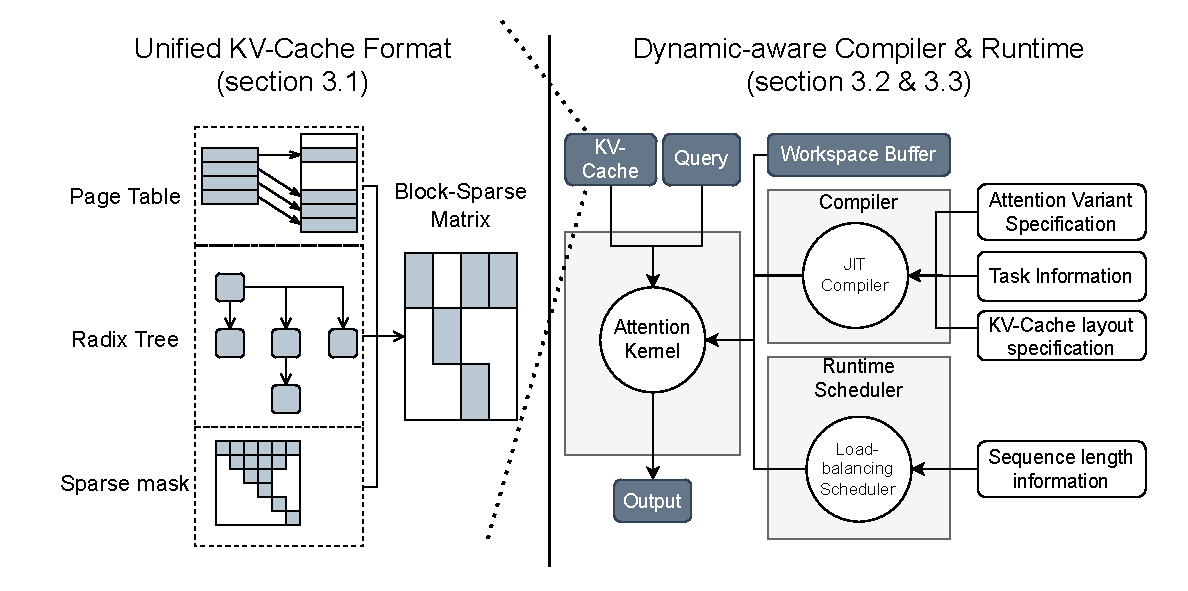
\includegraphics[width=0.85\textwidth]{figures/flashinfer-overview.pdf}
    \caption{\sys 系统设计概览：注意力变体规格、任务信息与 KV-cache 布局细节在编译期提供以进行 JIT 编译；序列长度信息在运行期输入以进行动态调度。}
    \label{fig:overview}
\end{figure*}

为 LLM 系统构建高效注意力支持主要面临两类挑战：

\textbf{LLM 应用呈现多样化工作负载模式与输入动态性。} LLM 服务涉及多种注意力计算模式，从上下文处理的 prefill 到在线服务中的批量解码~\cite{yu2022orca}。在多请求并发处理时，会出现\emph{前缀复用}机会；同时，推测式场景中的树解码会引入额外注意力模式~\cite{cai2024medusa,miao2023specinfer,chen2024sequoia}。此外，同一 batch 内及不同时间步之间的 query 长度与 KV cache 长度都在变化，朴素实现容易出现负载不均，因而需要内核具备动态自适应调度能力以达到最优性能。

\textbf{现代硬件实现要求注意力算子可定制。} 在内存侧，Paged Attention~\cite{kwon2023vllm}、Radix Tree~\cite{zheng2023sglang} 等高效存储格式对于管理不断增长的 KV cache 规模与多样存储模式至关重要。在计算侧，为充分释放不同 GPU 架构的性能潜力，需要构建架构特定的流水线与模板~\cite{dao2023flashattention2,jay2024flashattention3}。此外，现代 LLM 中注意力机制的变体也不断增加，例如分组注意力头~\cite{ainslie2023gqa, shazeer2019mqa}、特殊掩码~\cite{beltagy020longformer}、以及定制化的注意力分数计算~\cite{morgane2024gemma2,grok,jason2024flashsigmoid}，这要求实现策略同时具备灵活性与可扩展性。

工作负载多样性与硬件异构性的叠加，使得构建统一注意力方案变得复杂。当前各系统往往只覆盖上述特征的一个子集，导致维护成本高、效率潜力受限。为应对这些挑战，我们提出 \sys：一个基于代码生成的注意力引擎，旨在加速 LLM 中的注意力计算。其核心设计包括：

\textbf{\sys 使用块稀疏格式应对 KV-Cache 存储异构性。} 该格式可作为多类 KV-Cache 配置的统一数据结构，且可调块大小支持细粒度稀疏（如向量级稀疏）~\cite{chen2021tensorcoressparsity, li2022magicube}，从而统一多样 KV-Cache 模式并提升内存访问效率。

\textbf{\sys 提供可定制注意力模板以支持不同注意力变体。} 用户可通过可编程接口实现自身注意力变体；\sys 通过即时编译（JIT）将其转换为高度优化的块稀疏实现，以快速适配不同配置。

\textbf{\sys 采用动态负载均衡调度框架高效处理输入动态性。} 该框架将编译期 tile 大小选择与运行期调度解耦，提供轻量 API，在推理过程中随 KV-Cache 长度变化自适应调度，同时满足 CUDAGraph 对静态配置的要求~\cite{alan2019cudagraph, vinh2021pytorchcudagraph}。

图 \ref{fig:overview} 展示了我们的系统设计。我们在标准 LLM 服务场景与前缀共享、推测解码等创新场景下评估了 \sys 性能。\sys 已集成到 vLLM~\cite{kwon2023vllm}、MLC-Engine~\cite{mlcllm, lai2023relax}、SGLang~\cite{zheng2023sglang} 等主流 LLM 服务引擎。评测结果表明，\sys 在标准服务基准以及长上下文推理、并行生成等新场景中均带来显著的端到端时延与吞吐提升。

我们的贡献如下：
\begin{itemize}[itemsep=0pt,topsep=0pt,parsep=0pt]
    \item 提出灵活的块稀疏与可组合格式，应对 KV-Cache 存储异构性，实现高效内存管理与访问。
    \item 开发可定制注意力模板，支持多样注意力变体，并通过 JIT 编译保证高性能执行。
    \item 设计动态调度框架，在兼容 CUDAGraph 的同时处理输入动态性并最大化硬件利用率。
    \item 给出全面评估，展示内核级与端到端性能的显著提升。
\end{itemize}
\vspace{-1em}
